% -*- root: cuthesis_masters.tex -*-

\section{Introduction}
\label{chap3:sec:introduction}
Software companies and organizations have a common goal when developing software projects: both aim to deliver high-quality, useful software in a timely manner. However, in most practical settings, developers and development companies are saddled with deadlines, giving them every incentive to release earlier than the ideal date, were product quality alone taken into account. Such situations are all too common and in many cases force developers to take shortcuts \cite{kruchten2013technical} \cite{seaman2015technical}. Recently, the term \emph{technical debt} was coined to denote the phenomenon of ``doing something that is beneficial in the short term but will incur a cost later on''~ \cite{cunningham1993wycash}. Prior work has shown that practitioners cite numerous reasons for assuming technical debt, among them: rushing to compensate for delays and still deliver on time or to make deadlines for incorporating with a partner product before release, alleviating time-to-market pressure, and meeting customer demands in a time-sensitive industry~\cite{lim2012balancing}.


% People studied different aspects of TD
More recently, a study by Potdar and Shihab \cite{ICSM_PotdarS14} introduced a novel method of identifying technical debt reported by developers. This so-called "self-admitted technical debt", abbreviated SATD, is declared in developer source code comments. Prior work \cite{MTD15p9} has demonstrated that accrual of SATD is commonplace in software projects, where reviewing source code comments can identify different types of technical debt (e.g., design, defect, and requirement debt).

Intuition and general belief concur that inducing a technical debt, which many developers resort to in a time crunch, negatively impacts software maintenance and overall quality~\cite{zazworka2011investigating,spinola2013investigating,GuoSGCTSSS11,seaman2015technical,kruchten2013technical}. However, to the best of our knowledge, there is no empirical study that examines the impact of SATD on software quality. Such a study is critical since it will help us (i) confirm or refute entrenched preconceptions regarding the technique and (ii) better understand how to manage SATD.


Therefore, in this chapter, we investigate an empirical relation between SATD and software quality in five open-source projects. In particular, we examine whether (i) files with SATD have more defects compared to files without SATD, (ii) whether SATD changes introduce future defects, and (iii) whether SATD-related changes tend to be more difficult. We measured the difficulty of a change in terms of the amount of churn, number of files, number of modified modules in a change, and entropy of a change. Our findings show that: i) while it is true that SATD files have more bug-fixing changes in a number of the studied projects, in other projects, files without SATD have more defects, thus there is no clear relationship between defects and SATD; ii) SATD changes are associated with less future defects than non-technical debt changes; and iii) SATD changes (i.e., changes touching SATD files) are more difficult to perform. Our study indicates that although technical debt has negative effects, its impact is not related to defects, but rather to making the system more difficult to change in the future.


\section{Related Work}
\label{chap3:sec:related_work}
\todo{TBC}

\section{Approach}
\label{chap3:sec:approach}

The objective of our study is to investigate the relationship between SATD and software quality. We measure software quality in two ways. First, we employ the traditional measure of counting defects in a file and defect-inducing changes, which is in line with most prior studies ~\cite{Kamei-tse-2013,Kim-tse-2008,sliwerski-msr-2005}. In particular, we measure the number of defects in SATD-related files and the percentage of SATD-related changes that introduce future defects. Second, since technical debt is meant to represent the phenomenon of taking a short term benefit at the cost of paying a higher price later on, we employ as a second measure the difficulty of the changes related to SATD. In particular, we use the churn, number of files, number of directories and entropy of a change to quantify difficulty. We formalize our study with the following three research questions:


\begin{itemize}
	\vspace{0.2cm}
	\item {\bf RQ1:} Do files containing SATD have more defects than files without SATD? Do the SATD files have more defects after the introduction of the SATD?\\
	%\vspace{0.2cm}
	\item {\bf RQ2:} Do SATD-related changes introduce future defects?\\
	%\vspace{0.2cm}
	\item {\bf RQ3:} Are SATD-related changes more difficult than non-SATD changes?
	%\vspace{0.2cm}
\end{itemize}


To address our research questions we followed the general procedure enumerated in Figure \ref{fig:Process_overview}, which consists of the following steps. First, we mined the source code repositories of the studied projects (step 1). Then, we extracted  source code files at the level of each analyzed project (step 2). Next, we parse the source code and extract comments from the source code of the analyzed systems (step 3). At this point, we apply the comment patterns proposed by Potdar and Shihab~\cite{ICSM_PotdarS14} to identify SATD (step 4). Finally, we analyze the changes to quantify defects in files and use the SZZ algorithm to determine defect-inducing changes (step 5).

%and then linking them to the issue-tracker systems (steps 6). Finally, we generated the results and discussed them in detail (step 7).

\begin{figure}[t]
	\centering
	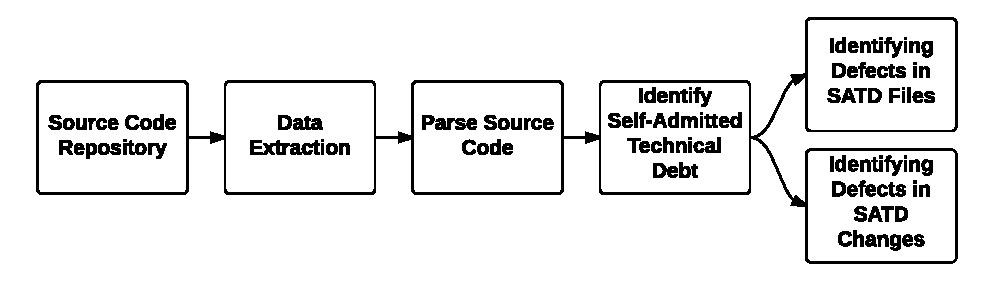
\includegraphics[width=150mm]{figures/chapter3/approach}
	\caption{Approach overview.}
	\label{fig:Process_overview}
\end{figure}


\subsection{Data Extraction}
Our study analyzes five large open-source software systems, namely Chromium, Hadoop, Spark, Cassandra, and Tomcat. We chose these projects because they represent different domains and programming languages (\ie{} Java, C, C++,  Scala, Python, and Javascript) and have a large number of contributors. More importantly, these projects are well-commented (since our approach for the detection of SATD is based on the source code comments). Moreover, they are all available to the research community as well as practitioners and have considerable development history.

Our analysis requires the source code as input. We downloaded the latest publicly available releases of the systems under consideration, \ie{} Chromium, Hadoop, Spark, Cassandra and Tomcat. Then, we filtered the data to extract the source code at the level of each project release. Files not consisting of source code (\eg{} CSS, XML, JSON) were excluded from our analysis as they do not contain the comments our analysis relies on.\\

Table~\ref{table:projects_statistics} summarizes the main characteristics of these projects. It reports (i) the release considered for each project, (ii) the date of the release, (iii) the number of lines of code for each release, (iv)  the number of comment lines, (v)  the number of source code files, (vi)  the number of committers, as well as (vii) the number of commits for each project release.

%\begin{landscape}
	
\begin{table*}[t]

		%\def\arraystretch{1.5}%

		\centering
		\caption{Characteristics of the studied projects.}
				\begin{adjustbox}{width=1.0\textwidth}
		\begin{tabular}{l|ll|ccccc}
			\hline
			\textbf{Project}  & \textbf{Release} & \textbf{ Release Date}  & \textbf{\# Lines of Code} & \textbf{\# Comment Lines} & \textbf{\# Files} & \textbf{\# Committers} & \textbf{\# Commits} \\ \hline
			\textbf{Chromium} &   45    & Jul 10, 2015 &  9,388,872   &    1,760,520    & 60,476 &    4,062    & 283,351  \\ \hline
			\textbf{Hadoop} &   2.7.1    & Jul 6, 2015 &  1,895,873   &    378,698    & 7,530 &    155    & 11,937  \\ \hline
			\textbf{Spark} &   2.3    & Sep 1, 2015 &  338,741   &    140,962    & 2,822 &    1,056    & 13,286  \\ \hline
			\textbf{Cassandra} &   2.2.2    & Oct 5, 2015 &  328,022   &    72,672    & 1,882 &    219    & 18,707  \\ \hline
			\textbf{Tomcat} &   8.0.27    & Oct 1, 2015 &  379,196   &    165,442    & 2,747 &    34    & 15,914  \\ \hline
		\end{tabular}
		\label{table:projects_statistics}
	\end{adjustbox}
\end{table*}

%\end{landscape}

\subsection{Scanning Code and Extracting Comments}
After obtaining the source code of the five software projects, we extracted the comments from their source code files. To this end, we developed a Python-based tool that identifies comments based on the use of regular expressions. This tool also indicates comment type (\ie{} single-line or block comments), the name of the file where the comment appears, and the line number of the comment. To ensure our tool's accuracy, we employ the Count Lines of Code (CLOC) tool~\cite{cloc}. As long as the total number of lines of comments is the same according to both tools, then the tool we developed is reliable.

In total, we found 879,142 comments for Chromium; 71,609 for Hadoop; 31,796 for Spark; 20,310 for Cassandra; and 39,024 for Tomcat. Of these, SATD comments numbered 18,435 for Chromium; 2,442 for Hadoop; 1,205 for Spark; 550 for Cassandra; and 1,543 for Tomcat. To enable easy processing of our data, we store all of our processed data in a PostgreSQL database, which we query to answer our RQs.


\subsection{Identifying Self-Admitted Technical Debt}
\label{td}
To perform our analysis, we need to identify SATD at two levels: (i) file level and (ii) change level.



\noindent\textbf{SATD files:} To identify SATD, we followed the methodology outlined in Potdar and Shihab~\cite{ICSM_PotdarS14}, who generated a list of 62 different patterns that indicate SATD. Therefore, in our approach, we determine which comments identify SATD by locating those that match any of the 62 patterns associated with SATD. These patterns are extracted from several projects and some appear more often than others. Examples of these patterns include \textit{``hack, fixme, is problematic, this isn't very solid, probably a bug, hope everything will work, fix this crap''}. The complete list of the patterns considered in this study is available online\footnote{http://users.encs.concordia.ca/\textasciitilde eshihab/data/ICSME2014/data.zip}.

Once we identify the comment patterns, we then abstract up to determine the SATD files. Files containing SATD comments are then labeled as {\em SATD files}, while files that do not contain any of these SATD comments are referred to as {\em non-SATD files}. We use these SATD files to answer RQ1.

\noindent\textbf{SATD changes:}
To study the impact of SATD at the change level, we need to identify SATD changes. To do so, we use our SATD files to determine the SATD changes. We analyze the changes and determine all the files that were touched by each change. If at least one of the files touched by the change is an SATD file, then we label that particular change as an SATD change. If the change does not touch an SATD file, then we label it as a non-SATD change. Table~\ref{table:satd_analyzed_projects} displays the percentage of SATD comments and files for each of the studied systems. From the table, we see that SATD comments exhaust less than 4\% of the total comments and between 10.17 and 20.14\% of the files are SATD files.

\begin{table}[tbh]
	\setlength{\tabcolsep}{.7\tabcolsep}
	\centering
	\caption{Percentage of SATD of the analyzed projects.}
	\begin{tabular}{l|c|c}
		\hline
		\textbf{Project}   & \textbf{SATD Comments (\%)} & \textbf{SATD files (\%)} \\ \hline
		\textbf{Chromium}  & 2.09             & 10.43                             \\ \hline
		\textbf{Hadoop}    & 3.41             & 18.59                             \\ \hline
		\textbf{Spark}     & 3.79             & 20.14                             \\ \hline
		\textbf{Cassandra} & 2.70             & 16.01                             \\ \hline
		\textbf{Tomcat}    & 3.95             & 10.17                             \\ \hline
	\end{tabular}
	\label{table:satd_analyzed_projects}
	\vspace{-0.2cm}
\end{table}
%\latifa {Did we apply SZZ, if yes we need a section on that as well - It is not clear whether it has been used or not}


\subsection{Identifying Defects in SATD Files and SATD Changes}
\label{bugs}
To determine whether a change fixes a defect, we search for co-occurrences of defect identifiers in change logs from the Git Version control system using regular expressions like ``fixed issue \#ID'', ``bug ID'',  ``fix'',  ``defect'',  ``patch'', ``crash'',  ``freeze'', ``breaks'', ``wrong'', ``glitch'', ``properly'', ``proper''.
Sliwersky \textit{et} al. \cite{sliwerski-msr-2005} showed that the use of such keywords in the change logs usually indicates the correction of a mistake or failure.
A similar  approach  was applied  to  identify  fault-fixing  and
fault-inducing  changes in  prior works  \cite{Kamei-tse-2013,Kim-tse-2008, sliwerski-msr-2005}. Once this step is performed, we identify, for each defect ID, the corresponding defect report from
the corresponding issue tracking system, \ie{} Bugzilla\footnote{https://www.bugzilla.org} or JIRA\footnote{https://www.atlassian.com/software/jira} and extract the relevant information from each report.

After grouping the SATD files and SATD changes, we proceed to identify the defects each contains. To do so, we follow the protocol previous research has adhered to in determining the number of defects in a file and locating defect-inducing changes~\cite{Kamei-tse-2013,Kim-tse-2008, sliwerski-msr-2005}.

\noindent\textbf{Defects in files:} Comparing the defectiveness of SATD and non-SATD files hinges on having the number of file defects at our disposal. To ensure this, we extract all the changes that have touched a file throughout the system's entire history. Then, we search for keywords in the change logs that indicate defect fixing as demonstrated in Figure~\ref{fig:indicating-a-bug-fixing-change}. A subset of the keywords we entered contains: ``fixed issue \#ID'', ``bug ID'',  ``fix'',  ``defect'',  ``patch'', ``crash'',  ``freeze'', ``breaks'', ``wrong'', ``glitch'', ``proper''. In cases where a defect identification is specified, we extract the defect report to verify that the defect corresponds to the system (\ie{} product).

Second, we establish whether the issue IDs identified in the change logs are true positives. Once we determine the defect fixing changes, we use these changes as an indication of the defect fixes that occur in a file, i.e., we count the number of defects in a file as the number of defect-fixing changes.


\noindent\textbf{Defect-inducing changes:} Similar to the process above, we first determine whether a change fixes a defect. To do so, we use regular expressions and specific keywords referencing a fix to search the change logs (i.e., commit messages) from the source code control versioning system. In particular, we search for the following keywords: ``fixed issue \#ID'', ``bug ID'',  ``fix'',  ``defect'',  ``patch'', ``crash'',  ``freeze'', ``breaks'', ``wrong'', ``glitch'', ``proper''. We also search for the existence of defect identification numbers in order to determine which defects, if specified, the changes actually fix.

Once we identify the defect-fixing changes, we map back (using the blame command) to determine all the changes that altered the fixed code in the past. Then, we determine the defect-inducing change as the change that is closest and before the defect report date. In essence, this tells us that this was the last change before a defect showed up in the code. If no defect report is specified in the fixing change, then following the precedent of prior work~\cite{Kamei-tse-2013}, we assume that the last change before the fixing change was the change that introduced the defect. This approach is often referred to as the SZZ~\cite{sliwerski-msr-2005} or approximate (ASZZ) algorithm~\cite{Kamei-tse-2013} and is to date the state-of-the-art in identifying defect-inducing changes.


\begin{figure}[h]
	\centering
	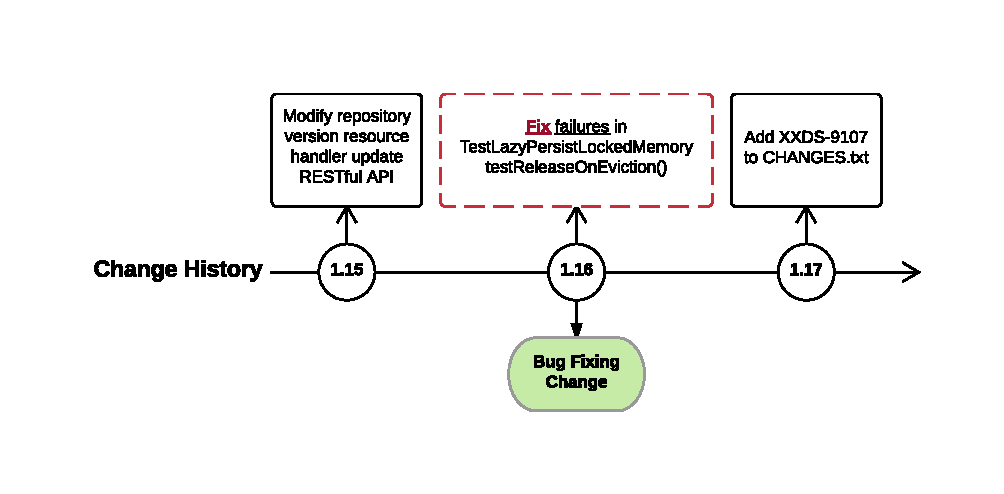
\includegraphics[width=150mm]{figures/chapter3/bug-fixing-change}
	\caption{Indicating a bug-fixing change.}
	\label{fig:indicating-a-bug-fixing-change}
\end{figure}



\section{Mann-Whitney-Wilcoxon Rank Sum Test}
The Mann-Whitney-Wilcoxon Rank Sum Test was used to analyze in the research \cite{mann1947test}. The test compared two groups of the same attribute for a data set and measured them to find any meaningful differences between them. This statistical test made use of median values for its comparison rather than mean values, allowing it to have the ability to characterize populations that do not follow a normal curve distribution. The main result of the test is the p-value it generates, which quantifies the probability of the null hypothesis being true, with the null hypothesis in this case being that both groups have the same central tendency. In our study we use this test to determine if the distinction between self-admitted technical debt and non-self-admitted technical debt files results in a difference in relevant statistical properties. If it does, then whatever caused a noticeable distinction between the files is meaningful to the statistical property. \iffalse After calculating how statistically significant the two sets are (\textbf{SATD vs. NSATD}) we proceed to perform our analysis, which we discuss in the next section.\fi \\




\section{Case Study Results}
\label{chap3:sec:results}

\begin{figure}[tb]
	\centering
	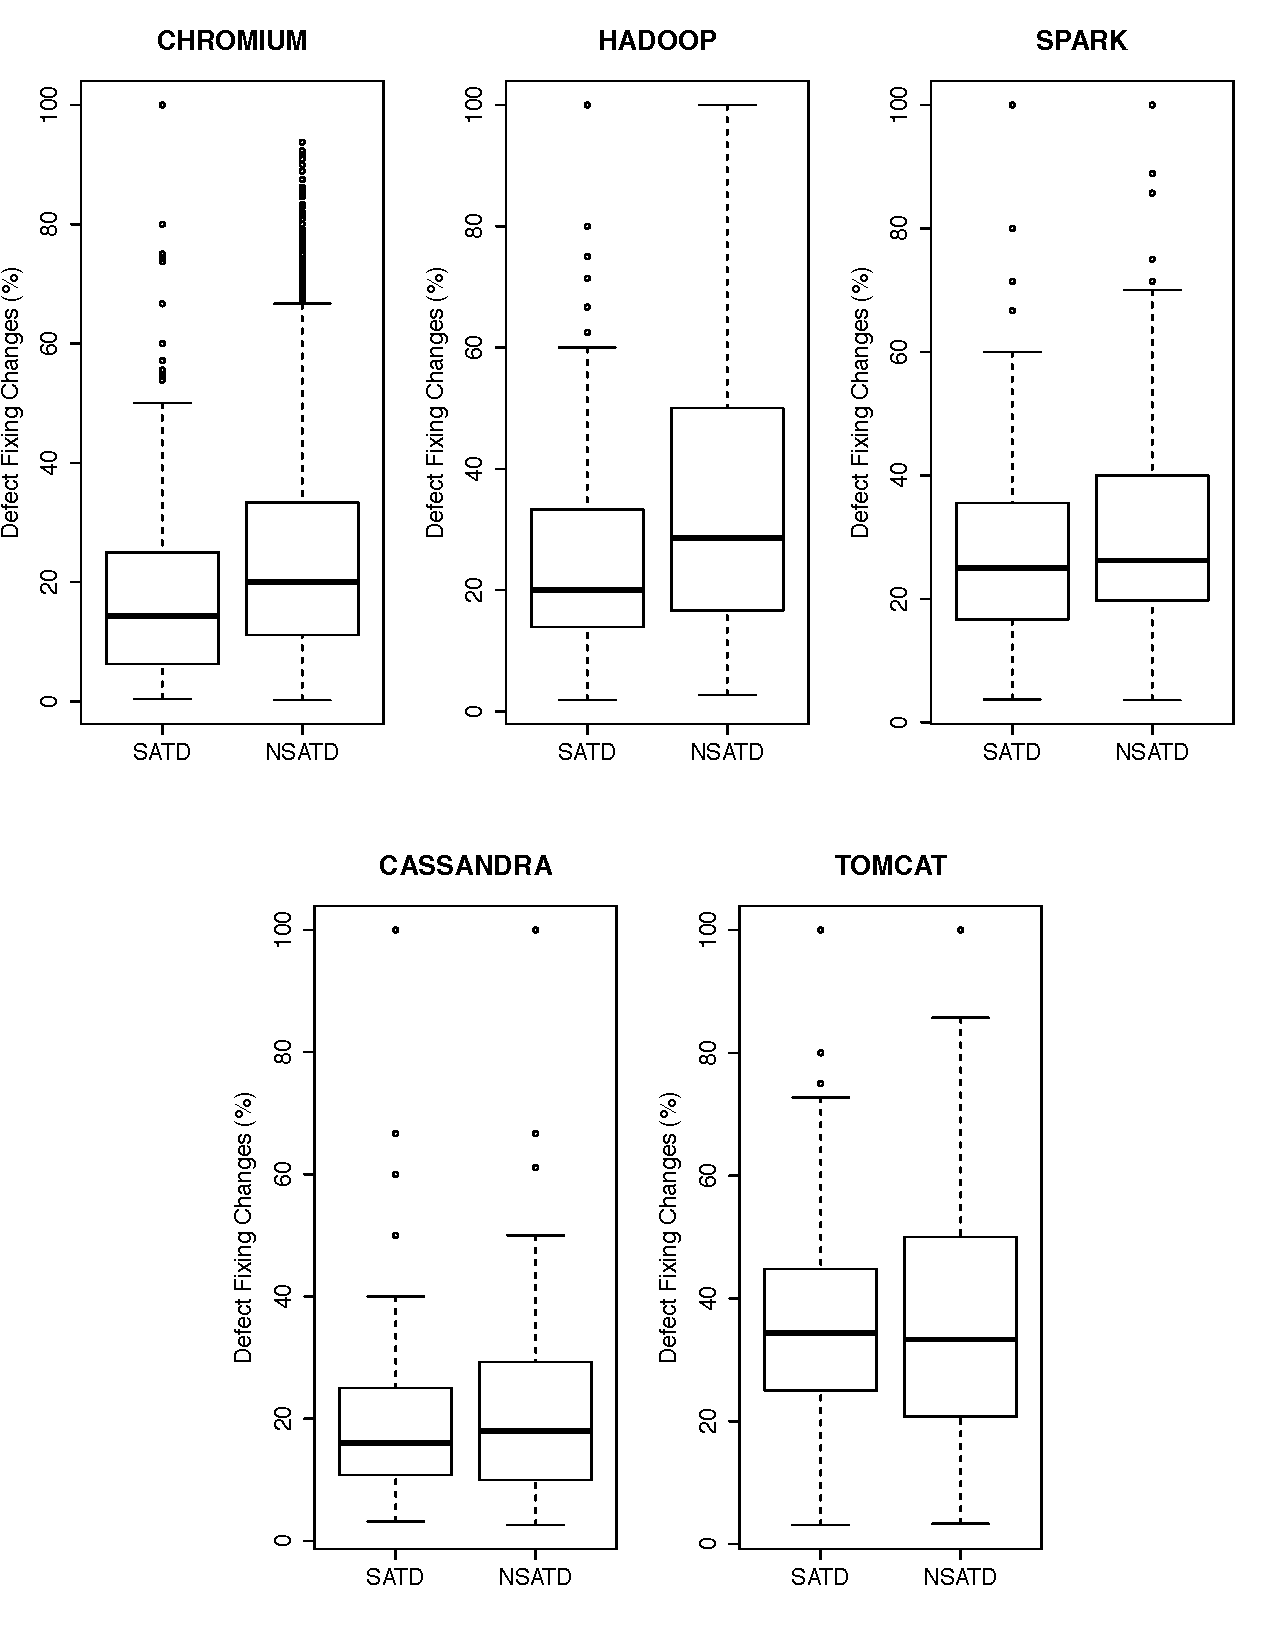
\includegraphics[width=90mm]{figures/chapter3/rq1_correction}
	\caption{Percentage of defect fixing changes for SATD and NSATD files.}
	\label{figure:number_of_fixing_changes_TD_vs_NTD}
\end{figure}

This section reports the results of our empirical study examining the relationship between self-admitted technical debt and software quality. 

For each project, we provide the descriptive statistics and statistical results, as well as a comparison with the other projects. 



In the following, we present for each RQ its motivation, the approach we took to address it, and our findings.


\subsection*{RQ1: Do files containing SATD have more defects than files without SATD? Do the SATD files have more defects after the introduction of the SATD?}

\noindent{\textbf{Motivation:}} Intuitively, technical debt has a negative impact on software quality. Researchers have studied technical debt and shown that it negatively impacts software quality~\cite{zazworka2011investigating}. However, this research has neglected SATD, which is prevalent in software projects according to past research \cite{ICSM_PotdarS14}.

Empirically examining the impact of SATD on software quality provides researchers and practitioners with a better understanding of such SATD, warns them of its future risks, and raises awareness of the obstacles or challenges it can pose.

In addition to comparing the defect-proneness of SATD and non-SATD files, we also compare the defect-proneness of SATD files before (pre-SATD) and after SATD (post-SATD). This analysis provides us with a different view of the defect-proneness of SATD files. In essence, it tells us whether the introduction of SATD is at all related to defects.



\begin{figure}[tb]
	\centering
	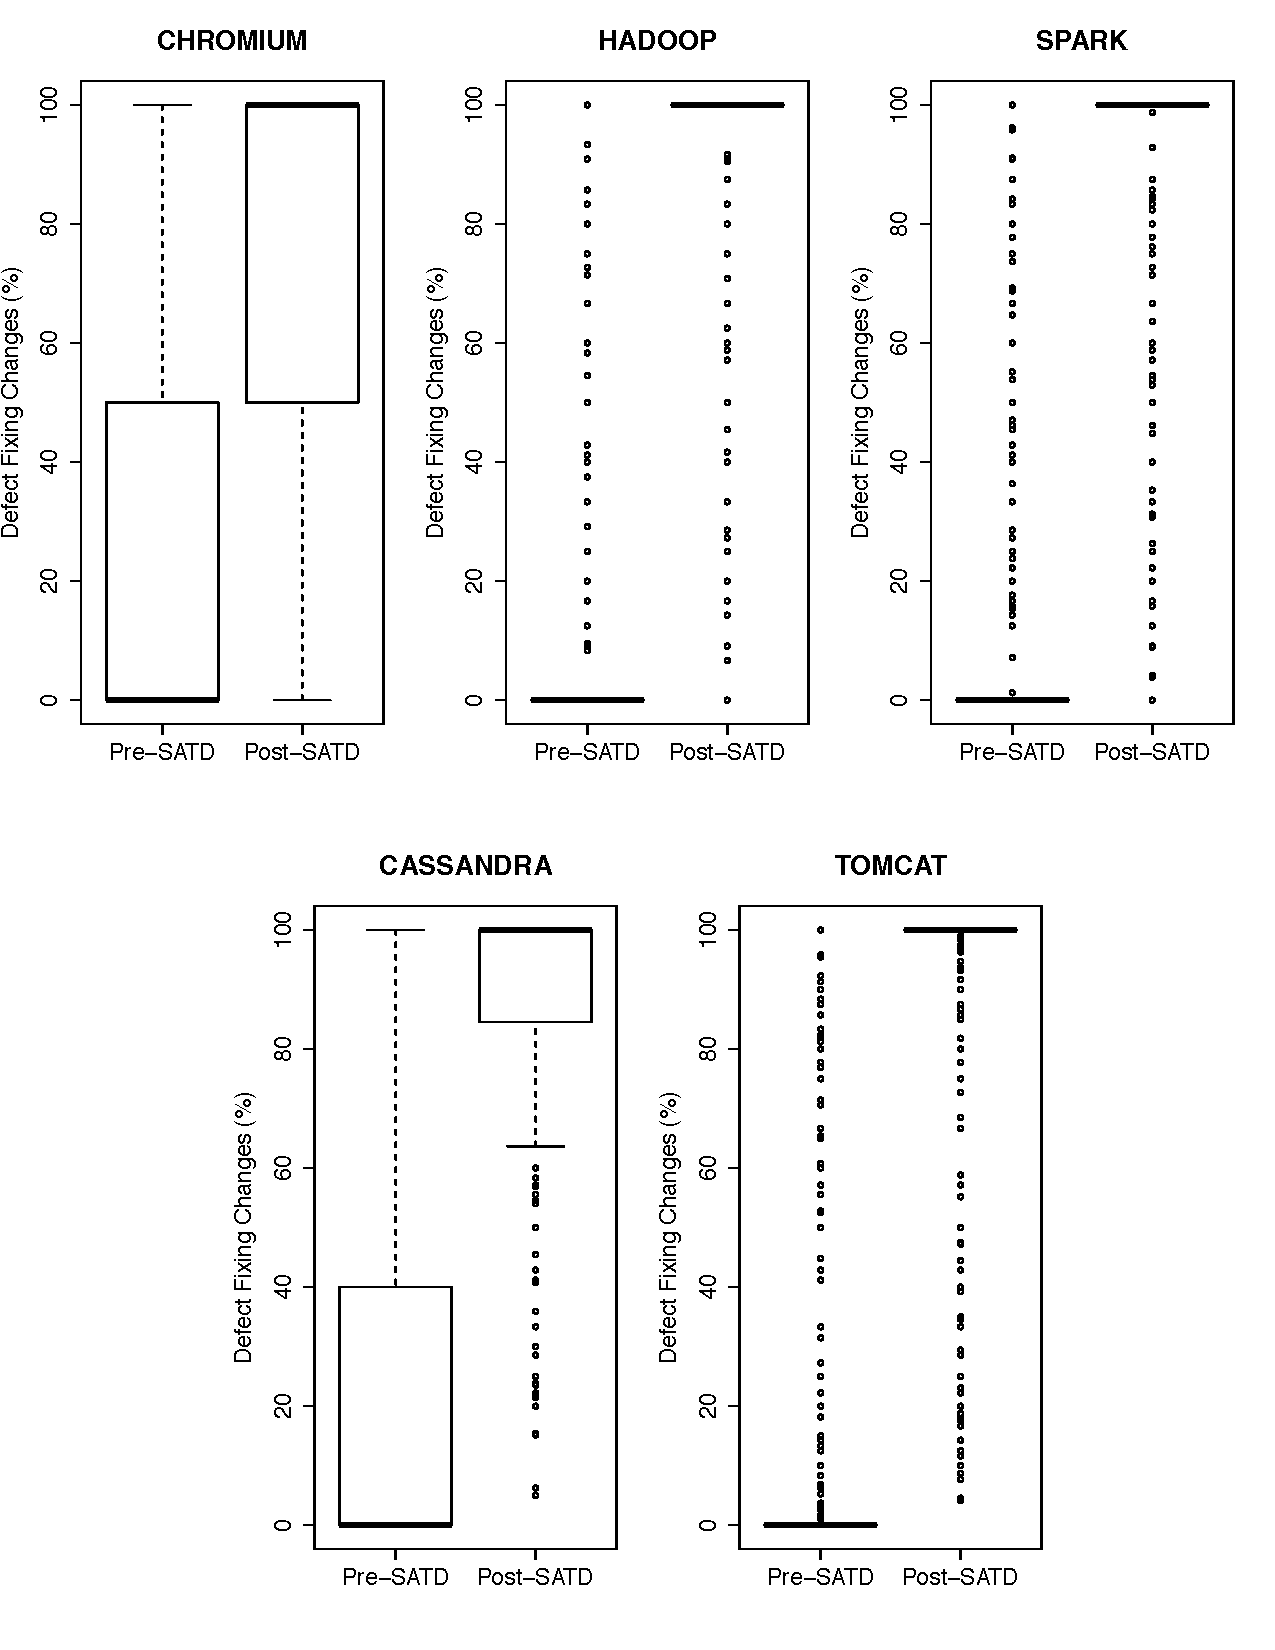
\includegraphics[width=90mm]{figures/chapter3/rq1-2_correction}
	\caption{Percentage of defect fixing changes for  pre-SATD and post SATD.}
	\label{figure:preVpost}
\end{figure}

\noindent{\textbf{Approach:}} To address RQ1, we perform two types of analyses. First, we compare the defect-proneness of files that do and do not contain SATD. Second, for the SATD files only, we compare defect-proneness before and after the introduction of SATD.

\noindent\textbf{Comparing SATD and non-SATD files.} To perform this analysis, we follow the procedure for identifying SATD files summarized earlier in Section ~\ref{td}. In a nutshell, we determine which files contain SATD comments and label them as SATD files. Files that do not contain any SATD are labeled as non-SATD files. Once we sort the files, we determine the percentage of defect-fixing changes in each file category (SATD and non-SATD). We opt for percentages over raw numbers so as to normalize our data since files can have different amounts of changes. To answer the first part of RQ1, we plot the distribution of defects by file category and perform statistical tests to compare their differences.

We perform the Mann-Whitney~\cite{mann1947test} test to determine if a statistical difference exists between the categories and Cliff's delta~\cite{Cliff:2005} to compute the effect-size. We use the Mann-Whitney test instead of other statistical difference tests because it is a non-parametric test that accommodates non-normal distribution (and as we will see later, our data is not normally distributed). We consider the results of the Mann-Whitney test to be statistically significant if the p-value is below $p <= 0.05$. In addition, we computed the effect-size of the difference using the Cliff's delta ($d$) non-parametric effect-size measure, which measures how often values in one distribution are larger than the values in another. Cliff's $d$ ranges in  the interval $[-1,1]$ and is considered small for $0.148 \le d < 0.33$, medium for $0.33 \le d < 0.474$, and large for $d \ge 0.474$.




\noindent\textbf{Comparing files pre- and post-SATD.} To compare SATD files pre- and post-SATD, we first determine all the changes that touched a file and then identify the change that introduced the SATD. Next, we measure the percentage of defects (i.e., $\frac{\#~of~fixing~changes}{total~\#~changes}$) in the file before and after the introduction of the SATD. We compare the percentage of defects instead of the raw numbers since SATD could be introduced at different times, i.e., we may not have the same total number of changes before and after the SATD-introducing change. Once we determine the percentage of defects in a file pre- and post-SATD, we perform the same statistical test and effect-size measure, \ie{} Mann-Whitney and Cliff's delta.


\noindent{\textbf{Results - Defects in SATD and non-SATD files:}} Figure \ref{figure:number_of_fixing_changes_TD_vs_NTD} shows  of the percentage of defect-fixing changes in SATD and non-SATD files for the five projects. We observe that in four out of five cases, the non-SATD (NSATD) files have a slightly higher percentage of defect-fixing changes: in Chromium, Hadoop, Spark and Cassandra. However, in Tomcat, SATD files have a slightly higher percentage of defects. For all projects, the $p$-values were $<0.05$, indicating that the difference is statistically significant. However, when we closely examine the Cliff's delta values in Table~\ref{table:cliff_deltas_RQ1}, we see a different trend for Chromium. In Chromium and Tomcat, SATD files often have higher defect percentages than non-SATD files and the effect-size is medium for Chromium and small for Tomcat. On the other hand, in Hadoop, Cassandra and Spark, SATD files have lower defect percentages than non-SATD files and this effect is large for Hadoop, medium for Cassandra and small for Spark.

Our findings here underscore that there is no clear trend when it comes to the percentage of defects in SATD vs. non-SATD files. In some projects, SATD files have more bug-fixing changes, while in others, it is the non-SATD files that have a higher percentage of defects.

\begin{table}[tb]
	\setlength{\tabcolsep}{.7\tabcolsep}
	\centering
	\caption{Cliff's Delta for SATD versus NSATD and POST versus PRE fixing changes.}
	\begin{tabular}{l|c|c}
		\hline
		\textbf{Project}   & {\bf SATD vs. NSATD} & {\bf Post- SATD vs. Pre- SATD} \\ \hline
		\textbf{Chromium}  & 0.407          & 0.704        \\ \hline
		\textbf{Hadoop}    & -0.562         & 0.137        \\ \hline
		\textbf{Spark}     & -0.221         & 0.463        \\ \hline
		\textbf{Cassandra} & -0.400         & 0.283        \\ \hline
		\textbf{Tomcat}    & 0.094          & 0.763        \\ \hline
	\end{tabular}
	\label{table:cliff_deltas_RQ1}
\end{table}

\noindent{\textbf{Results - Defects in pre- and post-SATD:}} Figure~\ref{figure:preVpost} shows boxplots for the percentage of defect-fixing changes in SATD files, pre- and post-SATD. Unsurprisingly, the post-SATD percentage of defect-fixing changes is higher for all projects. In Table~\ref{table:cliff_deltas_RQ1}, the effect-size Cliff's delta values corroborate our visual observations in that there is again more defect fixing post-SATD in the SATD files than pre-SATD. For all projects except Hadoop and Cassandra, where effect-size is small, the Cliff's delta is large.
%\latifa {any clues from the data or previous experience why this could be the case?}.


These findings contend that although it is not always clear whether SATD or non-SATD files will have a higher percentage of defects, there is a consistently higher percentage of defect-fixing once the SATD has been introduced.



\begin{figure}[tb!]
	\centering
	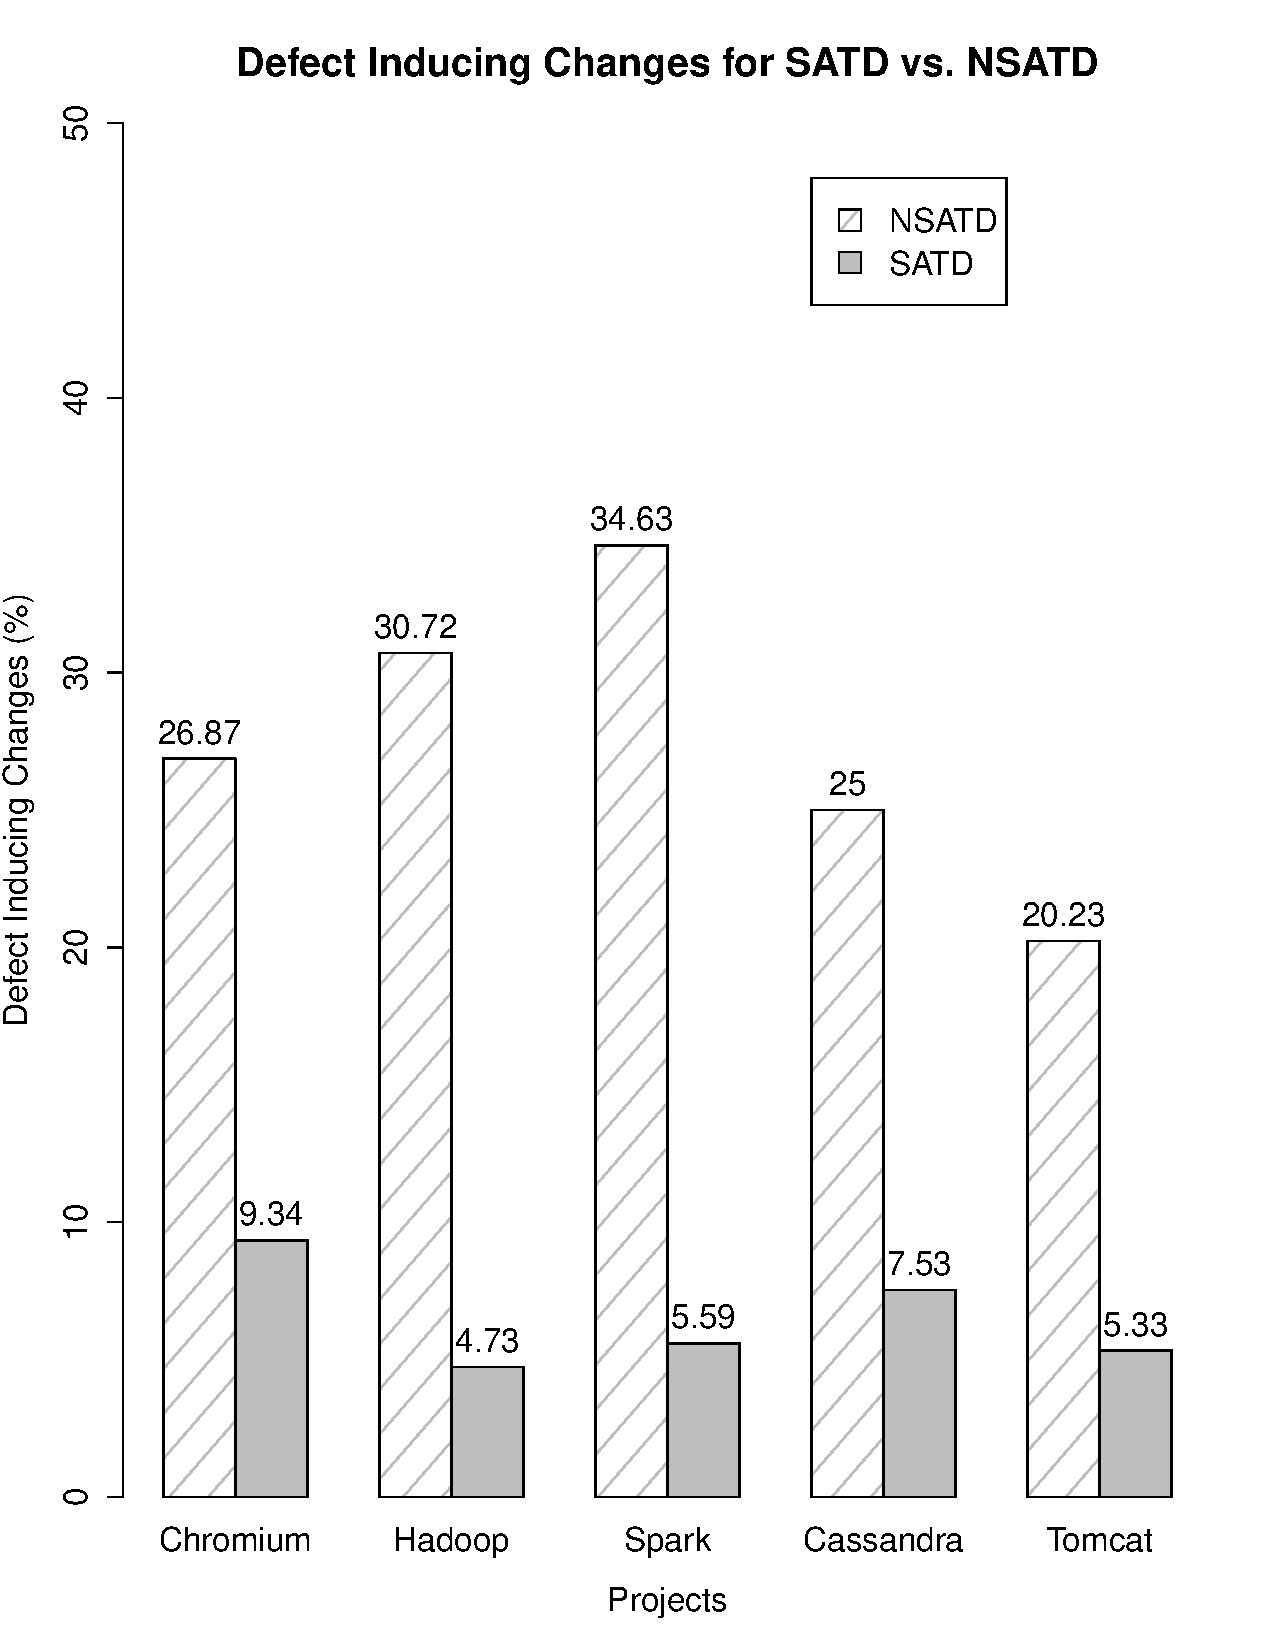
\includegraphics[width=90mm]{figures/chapter3/bug_inducing_changes}
	\caption{Percentage of defect inducing changes with SATD and NSATD.}
	\label{figure:bug_inducing_changes}
\end{figure}

\subsection*{RQ2: Do SATD-related changes introduce future defects?}

\noindent{\textbf{Motivation:}} After investigating the relationship between SATD and non-SATD at the file level, we would like to conclude whether the SATD changes are more likely to introduce future defects. Whereas the file-level analysis looked at files as a whole, our analysis here is more fine-grained and tailored to assess individual changes.

Studying the propensity of SATD changes to introduce future defects is important, as it informs us as to (i) how SATD and non-SATD changes compare in terms of future introduction of defects and (ii) how quickly the impact of SATD on quality can be felt. For example, if SATD changes introduce defects in the very next change, then this tells us that there is essentially no latent stage and the impact of SATD is felt almost immediately. Our conjecture is that SATD changes tend to be more complex and lead to the introduction of defects.


\noindent{\textbf{Approach:}}
To address RQ2, we applied the SZZ algorithm~\cite{sliwerski-msr-2005} to detect defect-inducing changes. Then, we sorted the results into two categories: SATD and non-SATD defect-inducing changes.




\noindent{\textbf{Results:}}
Figure \ref{figure:bug_inducing_changes} demonstrates that non-SATD changes have a higher incidence of defect-inducing changes relative to SATD changes.  In Chromium, for example, approximately 10\% of the SATD changes induce future defects, compared to roughly 27\% of the non-SATD changes. Our findings here show that contrary to our conjecture, SATD changes actually have a lower chance of inducing future defects.




\begin{table}[tb!]
	\setlength{\tabcolsep}{.7\tabcolsep}
	\centering
	\caption{Cliff's Delta for the change difficulty measures across the projects.}
	\begin{tabular}{l|C{1.5in}|c|c|C{2in}}
		\hline
		\textbf{Project}   & {\bf \# Modified Files}    & {\bf Entropy} & {\bf Churn} & {\bf\# Modified Directories}    \\ \hline
		\textbf{Chromium}  & 0.418 & 0.418   & 0.386 & 0.353 \\ \hline
		\textbf{Hadoop}    & 0.602 & 0.501   & 0.768 & 0.572 \\ \hline
		\textbf{Spark}     & 0.663 & 0.645   & 0.825 & 0.668 \\ \hline
		\textbf{Cassandra} & 0.796 & 0.764   & 0.898 & 0.827 \\ \hline
		\textbf{Tomcat}    & 0.456 & 0.419   & 0.750 & 0.390 \\ \hline
	\end{tabular}
	\label{table:cliff_deltas_RQ3}
\end{table}

\subsection*{RQ3: Are SATD-related changes more difficult than non-SATD changes?}

\noindent{\textbf{Motivation:}} Thus far, our analysis has confined itself to the relationship between SATD and software defects. However, by definition, technical debt entails some sort of tradeoff where a short-term benefit ends up costing more in the future. Therefore, it remains to be decided to what extent this tradeoff makes effecting changes more difficult after the introduction of technical debt.

Answering this question will help us understand the impact of SATD on future changes and provide us with a different view on how SATD impacts a software project.


\noindent{\textbf{Approach:}}  To answer this question, we classify the changes into two groups, \ie{} SATD and non-SATD changes. Then, we compare the difficulty of performing the two types of changes. We quantify the difficulty of a change using four different metrics: the total number of modified lines (\ie{} churn) in the change, the number of modified directories, the number of modified files and change entropy. The first three are motivated by earlier work on software decay by Eick \emph{et al.}~\cite{eick2001decay}, in which they measure decay. The change entropy metric is motivated by the work of Hassan~\cite{hassan2009predicting}, in which it measures change complexity.



To measure the change churn, number of files and number of directories, we use data from the change log directly. The churn is given for each file touched by the change, so we simply aggregate the churn of the individual files to determine the overall churn of the change. The list of files is extracted from the change log to determine the number of files and directories touched by the change. When measuring the number of modified  directories and files we refer to a directory as \textbf{ND} and  a file as \textbf{NF}. Hence, if a change involves the modification of a file having the path ``net/base/registry\_controlled\_domains/effective\_tld\_names.cc``, then the directory is \textit{base/registry\_controlled\_domains}, and the file is \textit{effective\_tld\_names.cc}.



\begin{figure}[!tb]
	\centering
	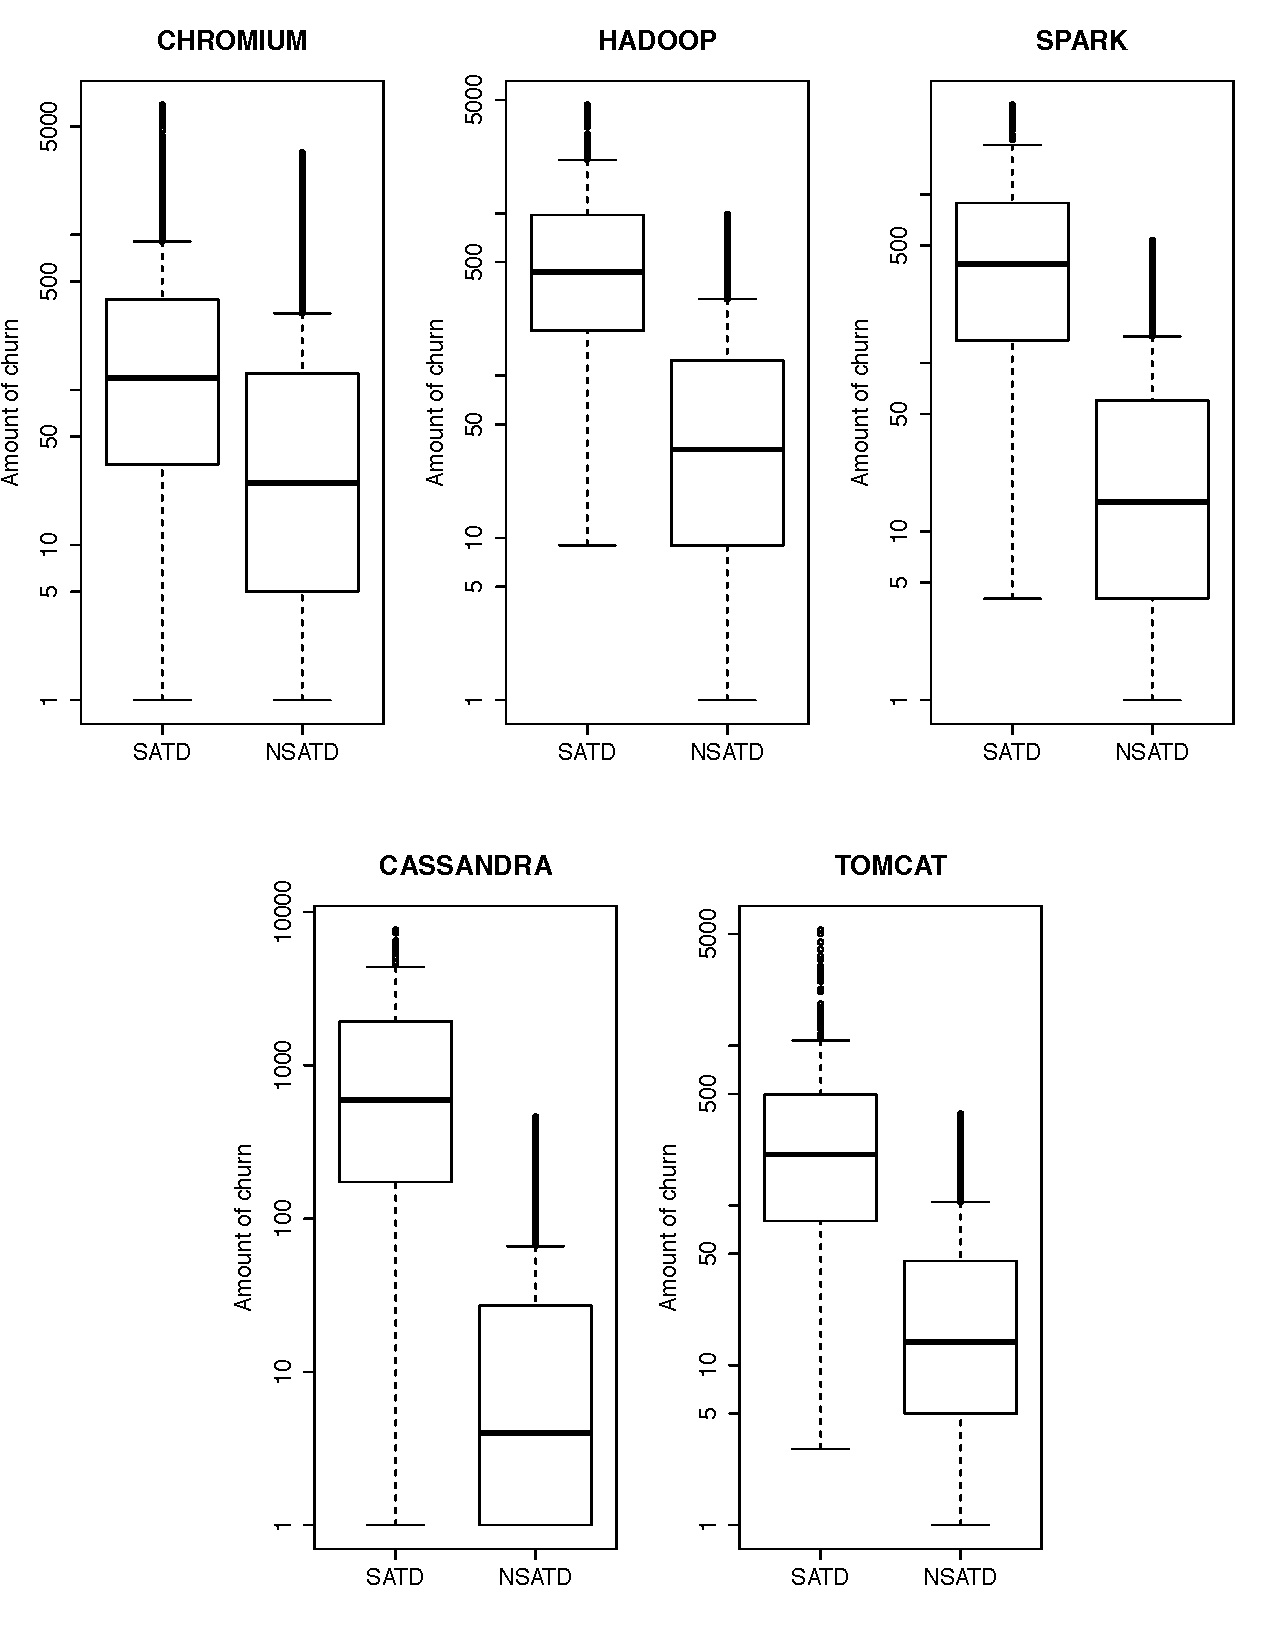
\includegraphics[width=90mm]{figures/chapter3/churn_for_all_projects}
	\caption{Total number of lines modified per change (SATD vs. NSATD).}
	\label{figure:tlcpc}
\end{figure}




\begin{figure}[!tb]
	\centering
	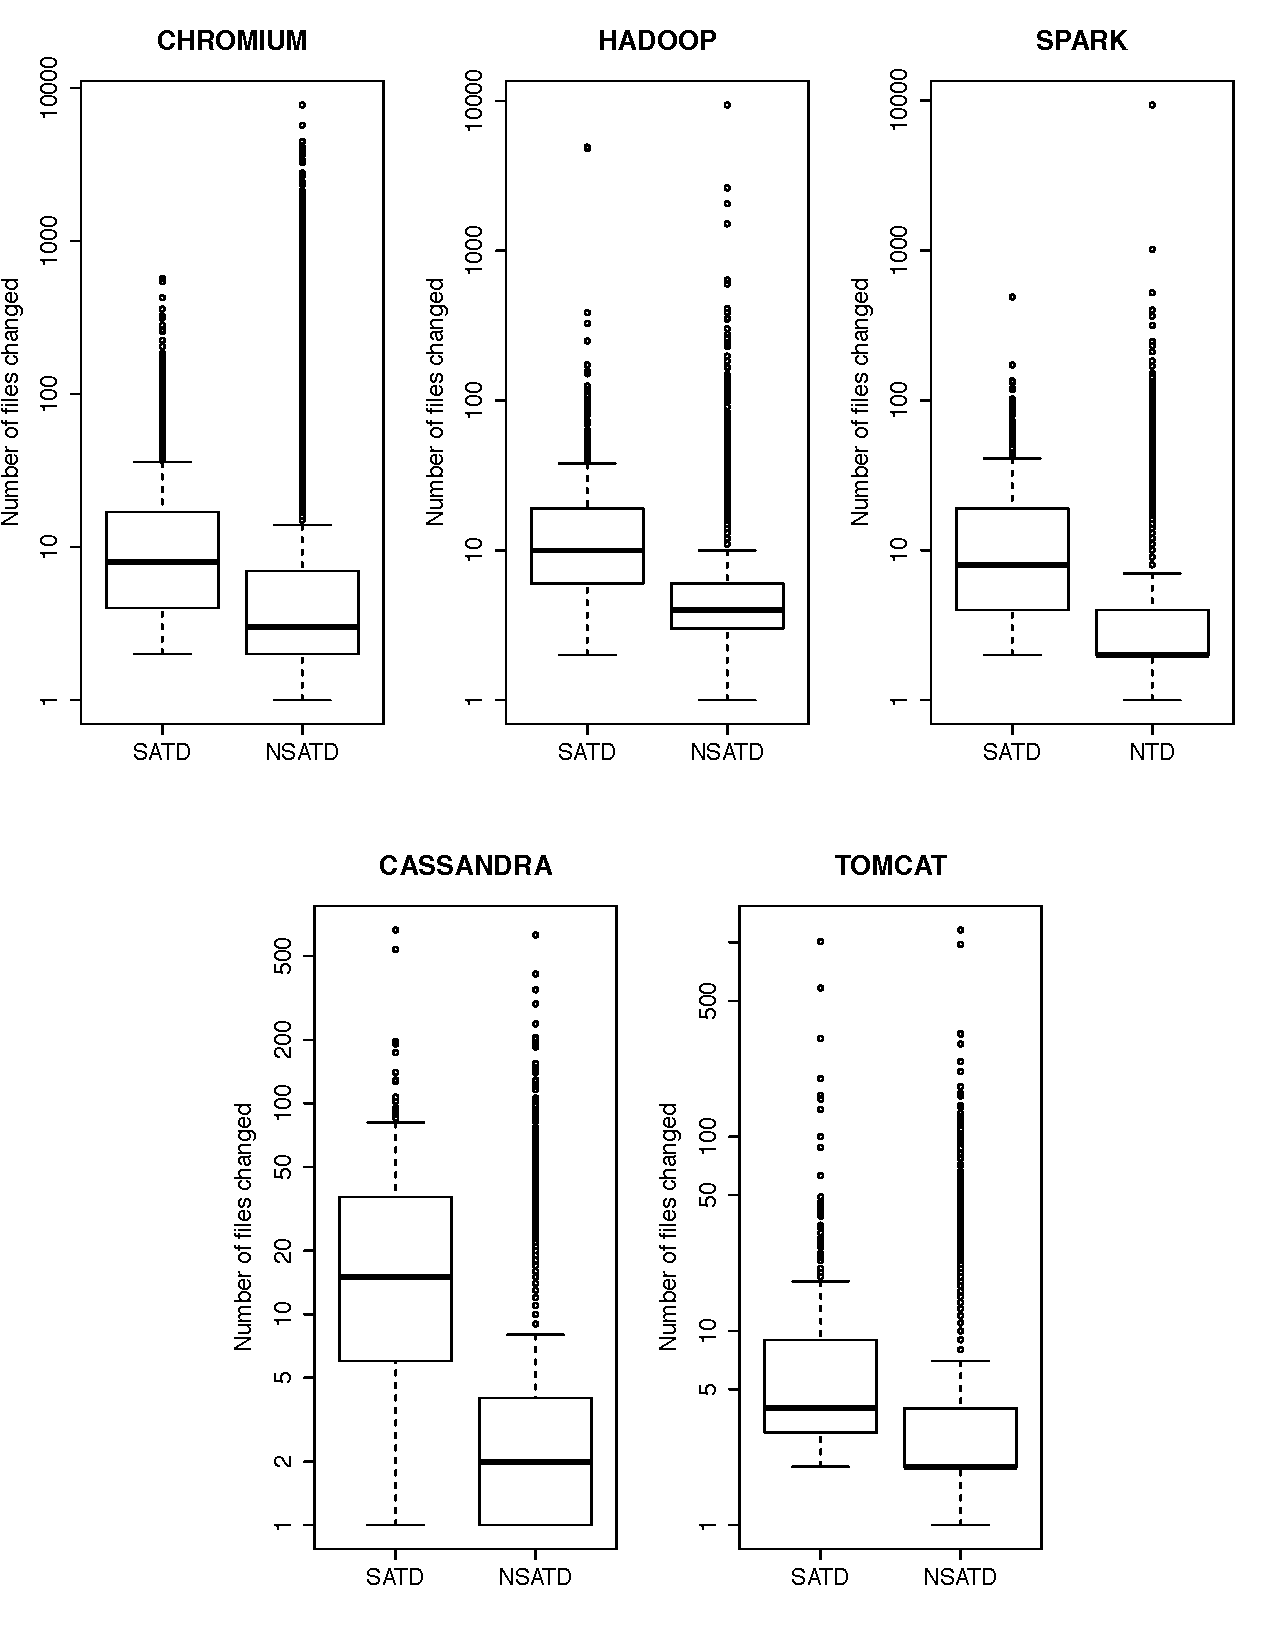
\includegraphics[width=90mm]{figures/chapter3/number_of_files_changed_all_projects}
	\caption{Total number of files modified per change (SATD vs. NSATD).}
	\label{figure:tfcpc}
\end{figure}

\begin{figure}[!tb]
	\centering
	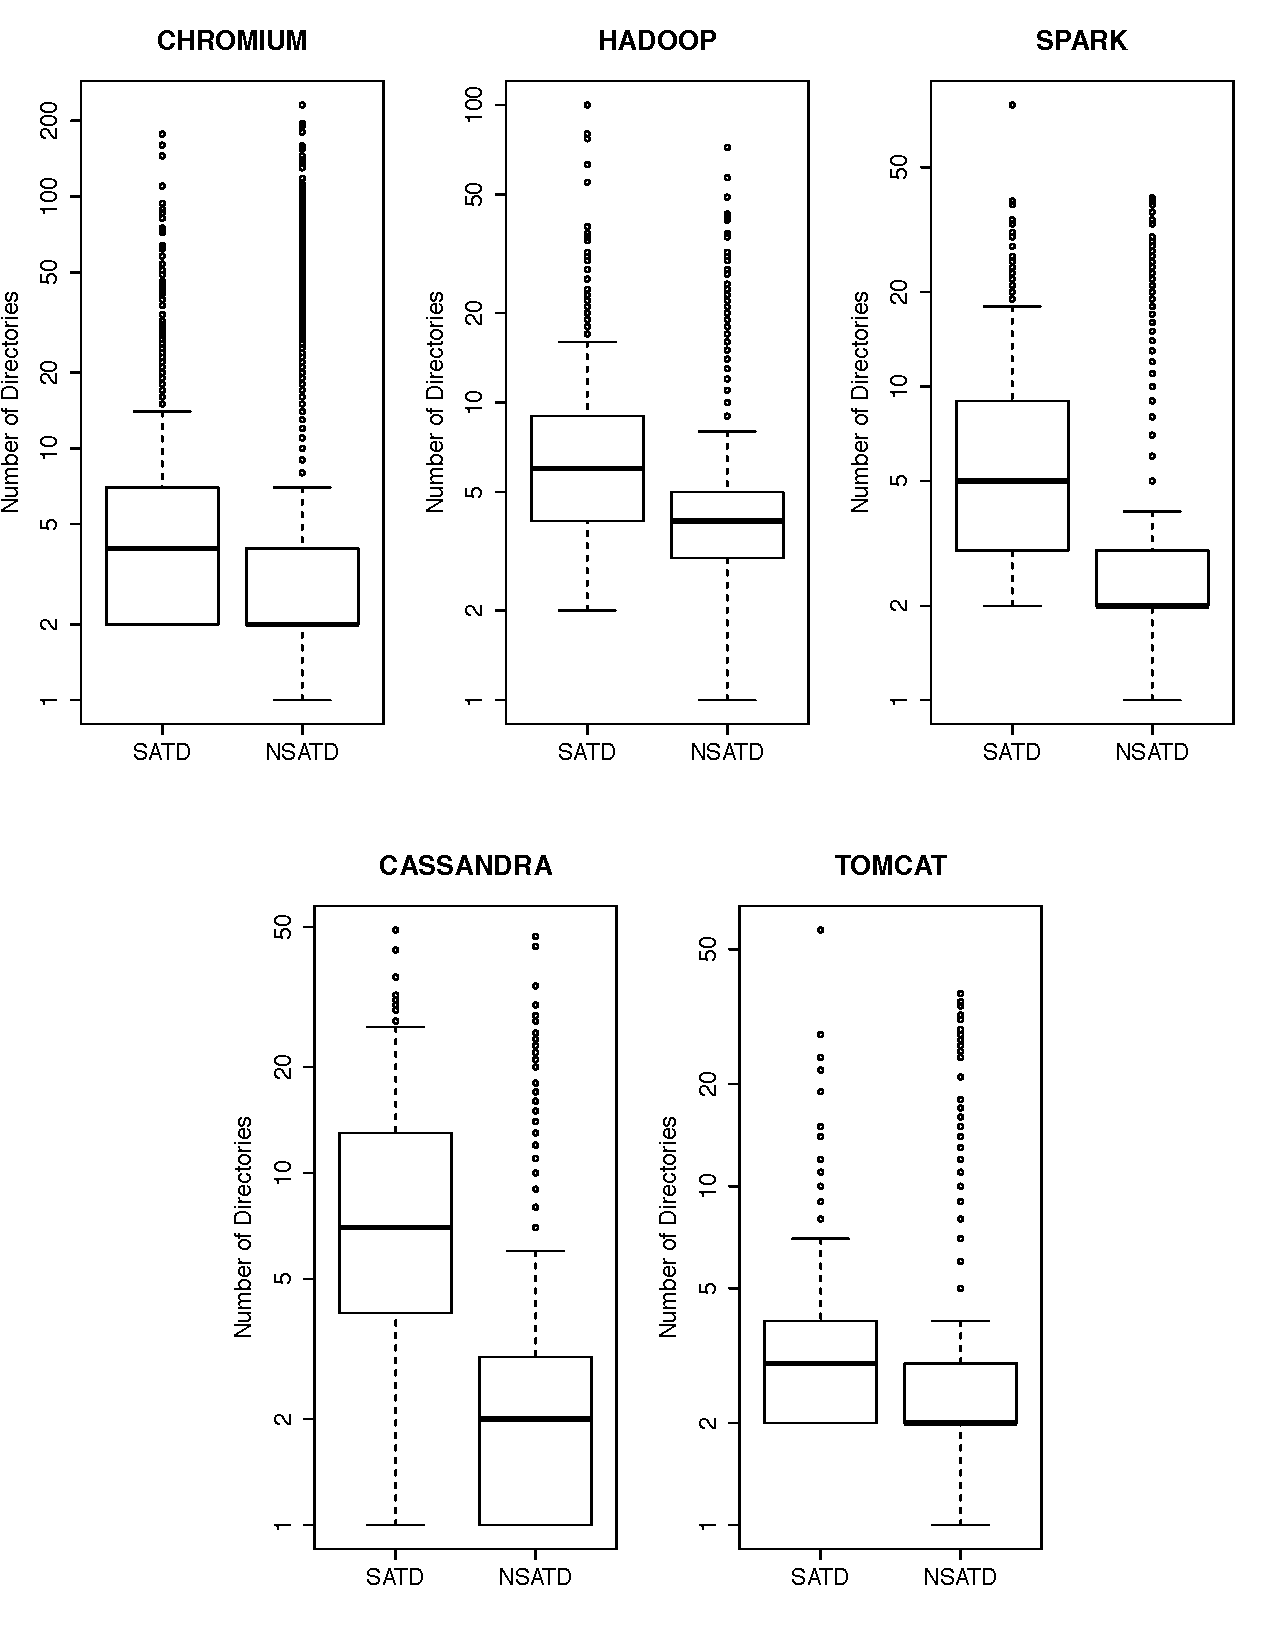
\includegraphics[width=90mm]{figures/chapter3/number_of_directories}
	\caption{Total number of modified directories per SATD and NSATD change.}
	\label{figure:number_of_directories}
\end{figure}


\begin{figure}[tb]
	\centering
	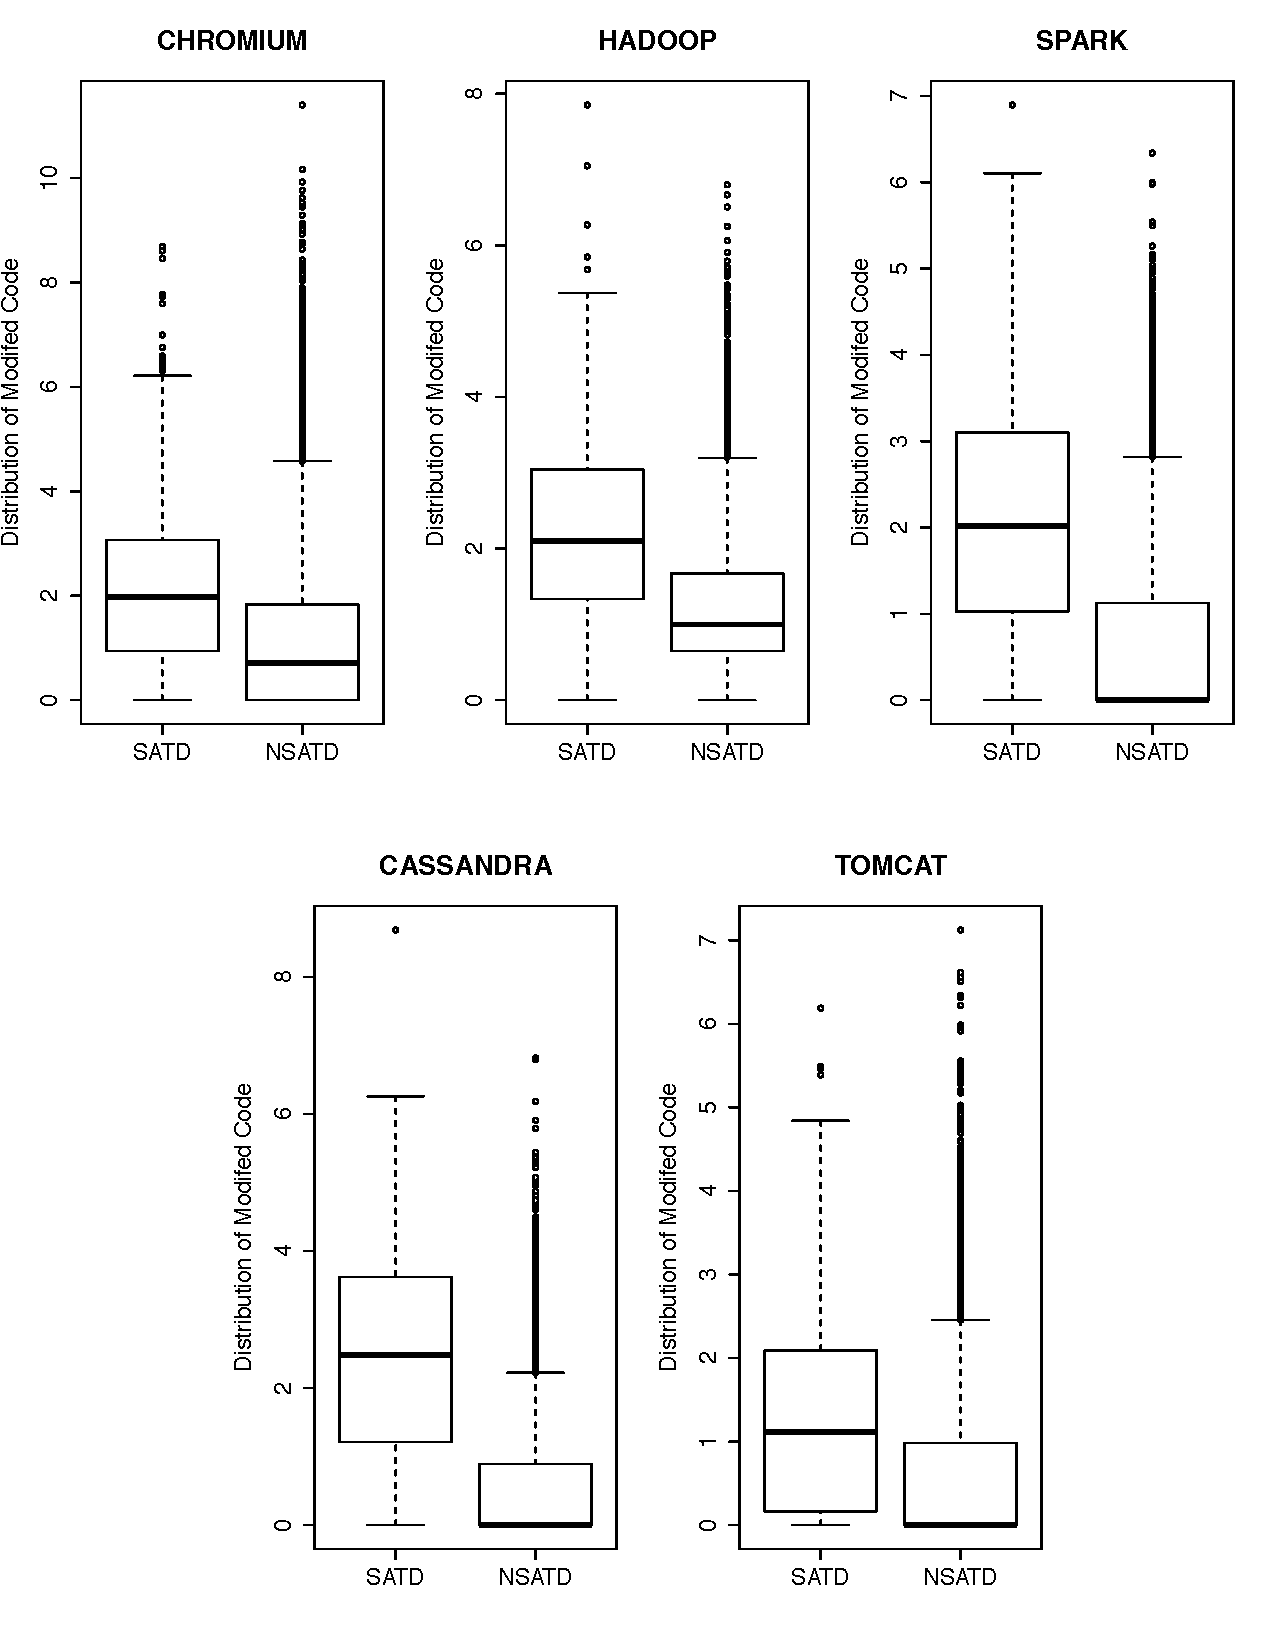
\includegraphics[width=90mm]{figures/chapter3/entropy_for_all_projects}
	\caption{Distribution of the change across the SATD and NSATD files.}
	\label{figure:mtdocatdf}
\end{figure}


To measure the entropy of the change, we use the change complexity measure proposed by Hassan~\cite{hassan2009predicting}. Entropy is defined as: $H(P)=-\sum _{k=1}^{n}\textrm ({p}_{k}*{log}_{2} {p}_{k})$, where $k$ is the proportion file$_{k}$ is modified in a change and $n$ is the number of files in the change. Entropy measures the distribution of a change across different files. Let us consider a change that involves the modification of three different files named \textit{A, B} and \textit{C} and let us suppose the number of modified lines in files\textit{ A, B} and \textit{C} is 30, 20, and 10 lines respectively. The entropy is equal to:
$(1.46=-\frac{30}{60}\log_{2}\frac{30}{60}-\frac{20}{60}\log_{2}\frac{20}{60}-\frac{10}{60}\log_{2}\frac{10}{60})$.

As in Hassan \cite{hassan2009predicting}, the above entropy formula has been normalized by the maximum entropy $log_{2}n$ to account for differences in the number of files per change. The higher the normalized entropy, the more difficult the change.




\noindent{\textbf{Results:}} Figures~\ref{figure:tlcpc},~\ref{figure:tfcpc},~\ref{figure:number_of_directories},~\ref{figure:mtdocatdf} reveal that for all difficulty measures, SATD changes have a higher value than non-SATD changes. We also find that the difference between the SATD and non-SATD changes is statistically significant, with a $p-value<0.05$. Table~\ref{table:cliff_deltas_RQ3} shows the Cliff's delta effect-size values for all projects studied. We observe that for all projects and all measures of difficulty, the effect-size is either medium or large (Cf. Table~\ref{table:cliff_deltas_RQ3}), which indicates that SATD changes are more difficult than non-SATD changes.

In summary, we conclude that SATD changes are more difficult than non-SATD changes, provided that difficulty is measured using churn, the number of modified files, the number of modified directories and change entropy.







\section{Threats to Validity}
\label{chap3:sec:threats_to_validity}

Threats  to {\bf  internal validity}  concern any factors that could have confounded our study results. To identify SATD, we use source code comments. In some cases, though, developers may not add comments when they introduce technical debt. The opposite poses another threat, namely, that developers might introduce technical debt and subsequently remove it without removing the related comment, i.e., the code and comment change inconsistently. However, Potdar and Shihab~\cite{ICSM_PotdarS14} examined this phenomenon in Eclipse and found that in 97\% of cases code and comments change in tandem. As a means of locating the SATD, we use the comments compiled by Potdar and Shihab~\cite{ICSM_PotdarS14}, yet there is a possibility that these patterns do not detect all SATD. Additionally, given that comments are written in natural language, Potdar and Shihab had to manually read and analyze them to determine those that would indicate SATD. Manual analysis is prone to subjectivity and errors and therefore we cannot guarantee that all considered patterns will be perceived as SATD indicators by other developers. To mitigate this threat, we manually examined each comment that we detected and verified that it contained one of the 62 patterns in \cite{ICSM_PotdarS14}. We performed this step, independently, for each of the five projects studied. We identify a change as an SATD change if it contains at least one SATD file. Alternatively, we could have defined SATD changes as only those for which all files have SATD. We elected to do it the former way because sometimes SATD in just one file can impact the rest of the change, e.g., cause many other files to be changed. When measuring the percentage of file defects after the introduction of SATD, it is difficult to distinguish the differences due to SATD from those attributed to natural evaluation of the files.



Threats  to {\bf external validity} concern the possibility that our results may not generalize. To optimize generalizability, we analyzed five large open-source systems and drew our data from the well-established, mature codebase of open-source software projects with well-commented source code. These projects belong to different domains, and they are written in different programming languages.


Furthermore, we focused on SATD only, which means that we do not cover all technical debt and therefore there may be other technical debt that is not self-admitted. Studying all technical debt is beyond the scope of this thesis.





\section{Conclusion and Future Work}
\label{chap3:sec:conclusion}



Technical debt is intuitively recognized as bad practice by software companies and organizations. However, there is very little empirical evidence on the extent to which technical debt can impact software quality. Therefore, in this thesis we perform an empirical study, using five large open-source projects, to determine precisely how technical debt relates to software quality. We focus on self-admitted technical debt, which refers to  errors that might be introduced due as part of intentional and temporary quick fixes. As in  \cite{ICSM_PotdarS14}, we leverage source code comments to identify such debt on the basis of recurring patterns that indicate its presence.


We examined the relationship between self-admitted technical debt and software quality by investigating (i) whether files with self-admitted technical debt have more defects compared to files without self-admitted technical debt, (ii) whether self-admitted technical debt changes introduce future defects and (iii) whether self-admitted technical debt-related changes tend to be more difficult. We measured the difficulty of a change in terms of the amount of churn, numbers of files and modified modules in a change, and change entropy.




Our findings suggest that there is no reliable trend when it comes to defects and self-admitted technical debt. In some of the projects, self-admitted technical debt files had more bug-fixing changes, while in others, files without it had more defects. We also found that self-admitted technical debt changes are less correlated with future defects than no technical debt changes, but more difficult to perform. 
\sultan{Our study demonstrates that although defects are not among the negative effects of technical debt, it can make the system more difficult to change in the future.}  Our study demonstrates that although technical debt may have negative effects, its impact does not extend to defects, rather making the system more difficult to change in the future.

We enlist empirical evidence in showcasing some of the drawbacks of technical debt that plague the software development process, in particular increases in system complexity. As a takeaway, practitioners would do well to keep technical debt in check and avoid its unwanted consequences. In the future, we intend to expound upon this research by studying the nature of defective SATD files more closely.
